\documentclass{beamer}

\usepackage[utf8]{inputenc}
\usepackage{amsfonts}
\usepackage{amsmath}
\usepackage{multicol}
\usepackage[noend]{algpseudocode}
\usefonttheme{serif}
\usetheme{Boadilla}
\usecolortheme{seahorse}

\title[Foraging]{Biomimicry of Bacterial Foraging}
\subtitle{for Distributed Optimization and Control}
\author[Passino, by Van de Kleut]{
  Kevin M. Passino\inst{1}\\
  Presented by: Alexander Van de Kleut\inst{2}
}
\institute{\inst{1}
  The Ohio State University\\
  Electrical and Computer Engineering
  \and
  \inst{2}
  University of Waterloo\\
  Centre for Theoretical Neuroscience
}
\date[W20]{IEEE Control Systems Magazine, 2002}

\begin{document}

\frame{\titlepage}

\begin{frame}
\frametitle{Table of Contents}
\tableofcontents
\end{frame}

% Kevin Passino is a professor of Electrical and Computer Engineering at Ohio State University.
% His work covers a broad range of disciplines, from virtual reality for mental health therapy to fuzzy control theory to humanitarian engineering.
% He has done considerable work on biomimicry and swarm intelligence.
% I've included here two selected textbooks he has been a major contributor for: Swarm Stability and Optimization, and Biomimicry for Optimization, Control, and Automation
% The paper I'm presenting today is Passino's second most-cited paper at over 3000 citations.
\section{About the Author}
\begin{frame}
\frametitle{About the Author}
\begin{columns}
  \column{0.5\textwidth}
    \includegraphics<1-2>[scale=2]{assets/kpassino}%
  \column{0.5\textwidth}
    \includegraphics<1>[scale=2]{assets/book1}
    \includegraphics<1>[scale=0.18]{assets/book2}
    \includegraphics<2>[scale=0.3]{assets/citations}
\end{columns}
\end{frame}

\section{Foraging}
\begin{frame}
\frametitle{Foraging}
\textbf{Foraging}
\begin{itemize}
  \item searching for nutrients
  \item avoiding noxious stimuli (toxins, predators, etc)
\end{itemize}
\textbf{Social Foraging}
\begin{itemize}
  \item increases likelihood of finding nutrients
  \item better detection and protection from noxious stimuli
  \item gains can offset cost of food competition
\end{itemize}
\end{frame}

\begin{frame}
\frametitle{Foraging as Optimization}
\textbf{How can we view foraging as an Optimization Process?}
\begin{itemize}
  \item<1-> We have some parameters $\theta$ and a loss function $J(\theta)$ that we want to minimize
  \item<2-> $\theta$ can represent the position of an organism in its environment
  \item<3-> $J$ can represent the concentration of nutrients and noxious stimuli
  \begin{itemize}
    \item smaller values of $J$ = more nutrients, less noxious stimuli
    \item higher values of $J$ = more noxious stimuli, less nutrients
  \end{itemize}
  \item<4-> In general, $J$ and $\theta$ can be arbitrary
  \begin{itemize}
    \item $\theta \in \mathbb{R}^p$
    \item $J: \mathbb{R}^p \to \mathbb{R}$
  \end{itemize}
\end{itemize}
\end{frame}

\section{Biological and Computational Model}
\begin{frame}
\frametitle{\textit{E. coli}}
\begin{itemize}
  \item<1-> Model organism
  \begin{itemize}
    \item<2-> Highly studied
    \item<3-> Well-characterized foraging behaviour
    \item<4-> Probably won't feel bad about simplifying its behaviour
  \end{itemize}
  \item<5-> Social organism
  \begin{itemize}
    \item<6-> Secretes signals to attract others nearby
    \item<7-> Encourages ``swarming'' or ``clumping''
  \end{itemize}
\end{itemize}
\end{frame}

\begin{frame}
\frametitle{\textit{\textit{E. coli}} Behaviour}
\begin{itemize}
  \item Swims using left-handed helical flagella (``propellers'')
  \begin{itemize}
    \item \textbf{Tumble}: flagella all rotate clockwise $\to$ pull on cell in all directions $\to$ random movement
    \item \textbf{Run}: flagella all rotate counterclockwise $\to$ flagella form a bundle $\to$ push on cell in one direction $\to$ directed movement
  \end{itemize}
\end{itemize}
\begin{center}
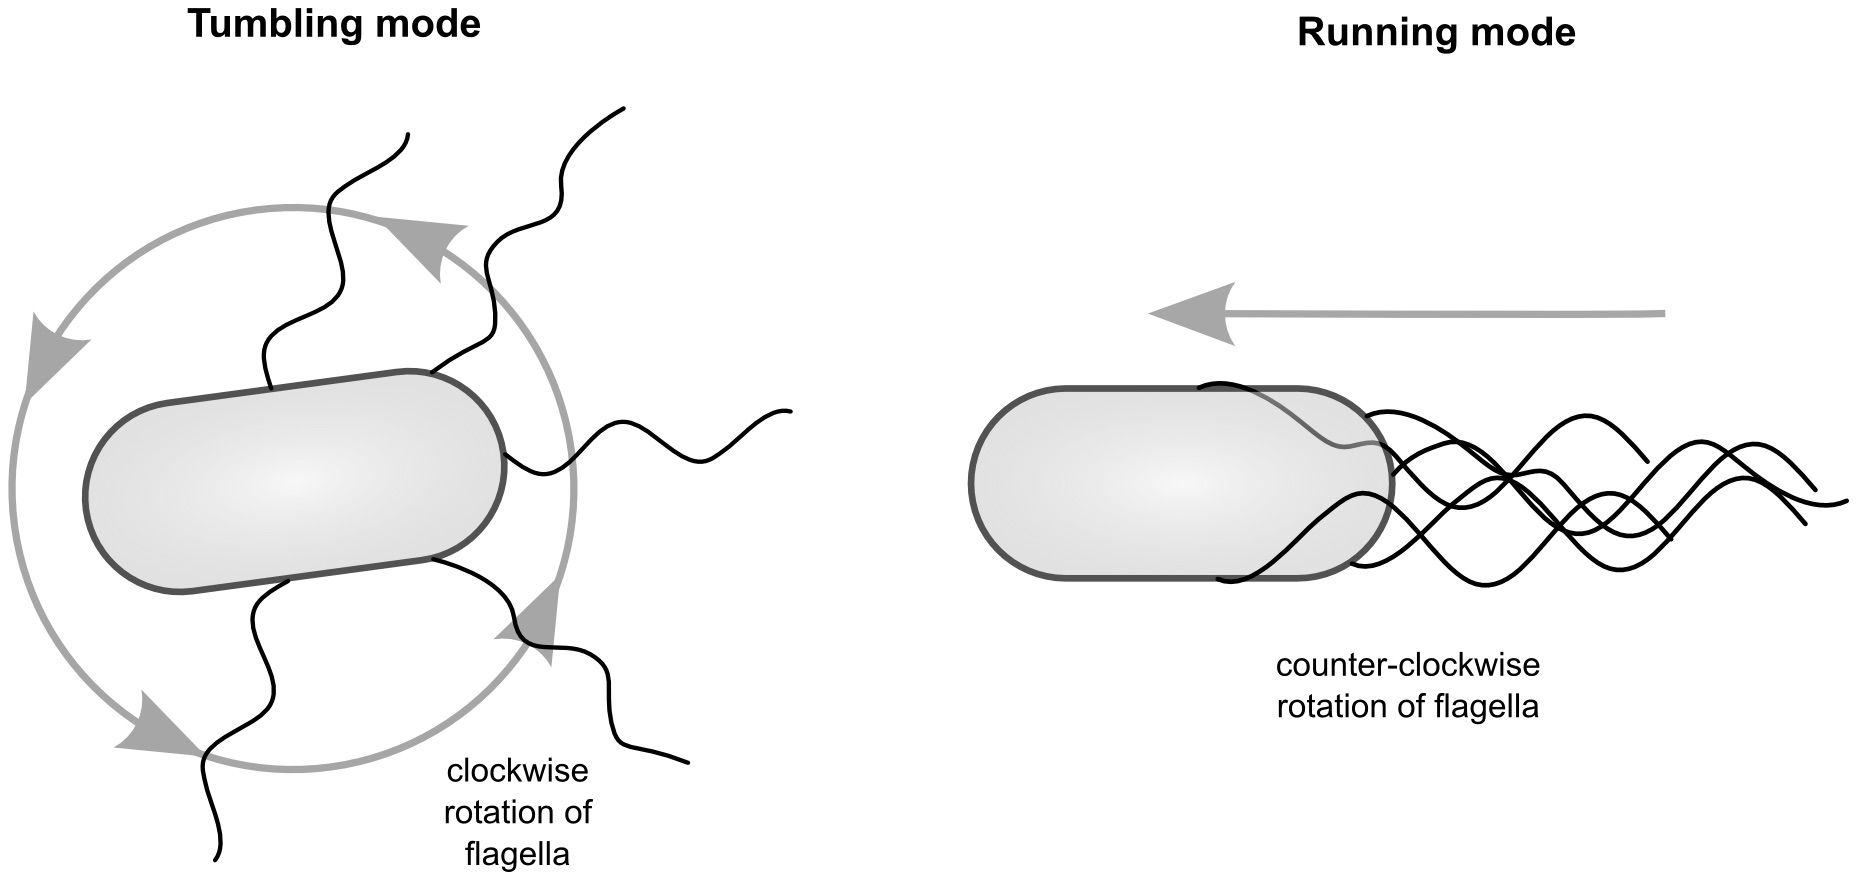
\includegraphics[scale=0.2]{assets/ecoli}
\end{center}
\end{frame}

\begin{frame}
\frametitle{\textit{\textit{E. coli}} Behaviour}
\begin{itemize}
  \item If during a tumble \textit{\textit{E. coli}} swims down a nutrient concentration gradient:
  \begin{itemize}
    \item Prolongs time spent on a run
    \item Continues moving in the same direction
  \end{itemize}
  \item Otherwise:
  \begin{itemize}
    \item Tends to switch to a tumble (search for more)
    \item Moves randomly which searching for more nutrient gradients to exploit
  \end{itemize}
  \item Call a tumble followed by a run a ``chemotaxis step''
\end{itemize}
\end{frame}

\begin{frame}
\frametitle{Algorithm for a Single Bacterium}
\begin{algorithmic}[1]
\For {$j \gets 1 \dots N_c $}:
  \State $\phi \sim \mathcal{U}$
  \State $\theta \gets \theta + c \phi$
  \While {$J(\theta + c \phi) < J(\theta)$}:
    \State $\theta \gets \theta + c \phi$
  \EndWhile
\EndFor
\end{algorithmic}
\begin{itemize}
  \item $\theta$: $p$-dimensional vector (randomly initialized)
  \item $N_c$: number of chemotaxis steps
  \item $\phi \sim \mathcal{U}$: a random unit vector
  \item $c$: a step-size
\end{itemize}
\end{frame}

\begin{frame}
\frametitle{Loss Function to Optimize}
\begin{columns}
\column{0.5\textwidth}
\begin{center}
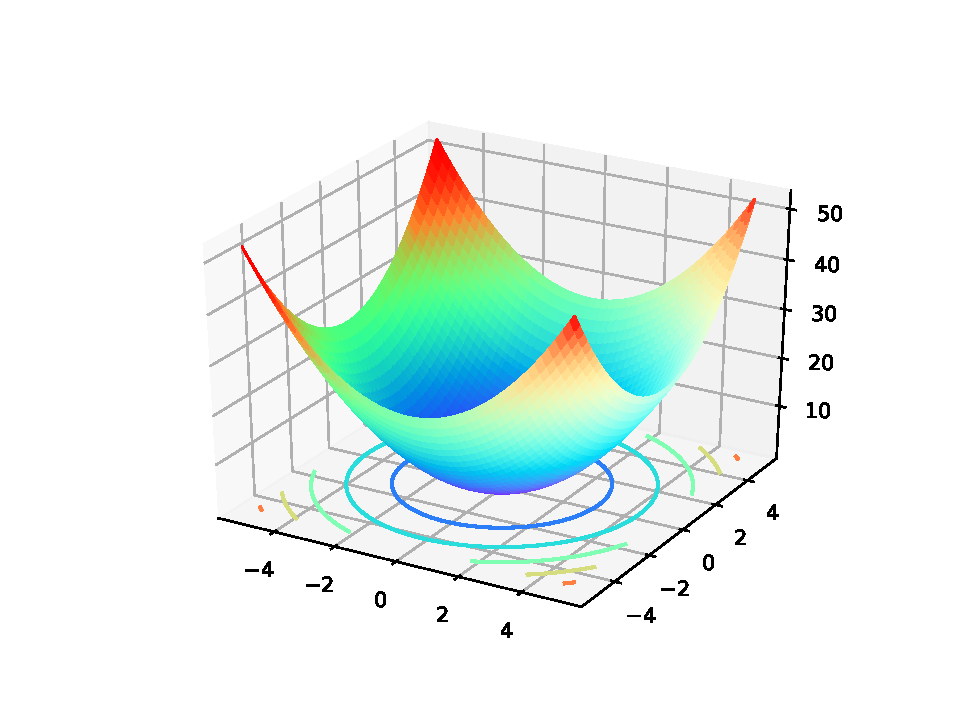
\includegraphics[scale=0.3]{assets/sphere}
\end{center}
\column{0.5\textwidth}
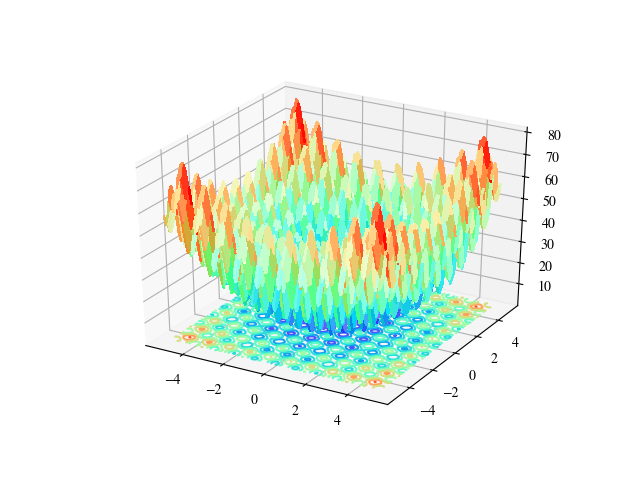
\includegraphics[scale=0.3]{assets/rastrigin}
\end{columns}
\end{frame}

\begin{frame}
\frametitle{Results of Single Bacterium}
\begin{columns}
  \column{0.5\textwidth}
    \begin{center}
      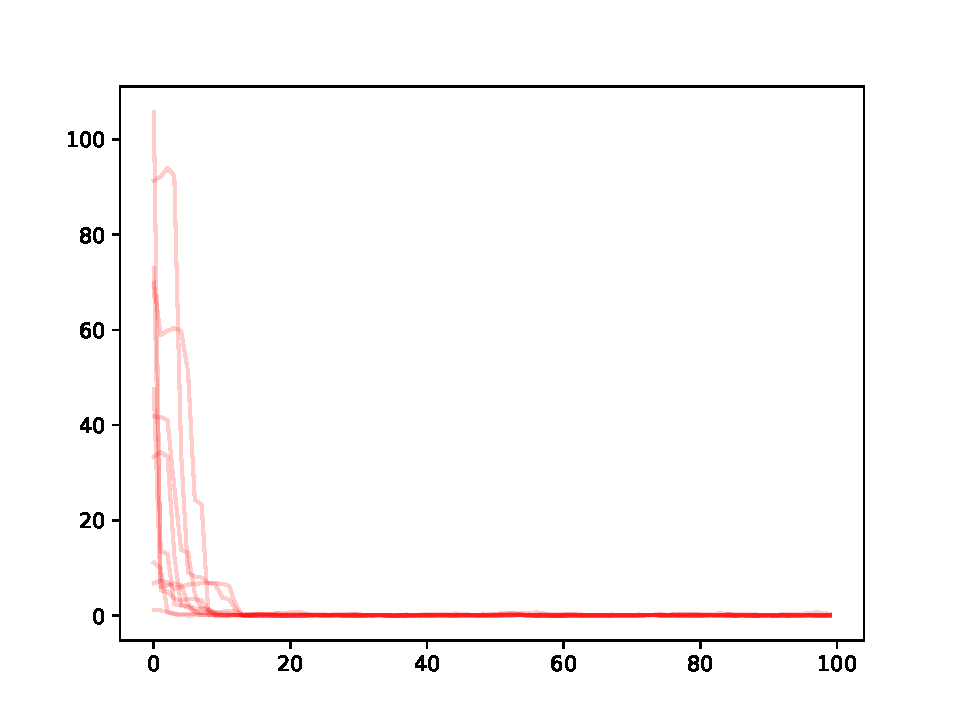
\includegraphics[scale=0.3]{assets/sphere_J}
      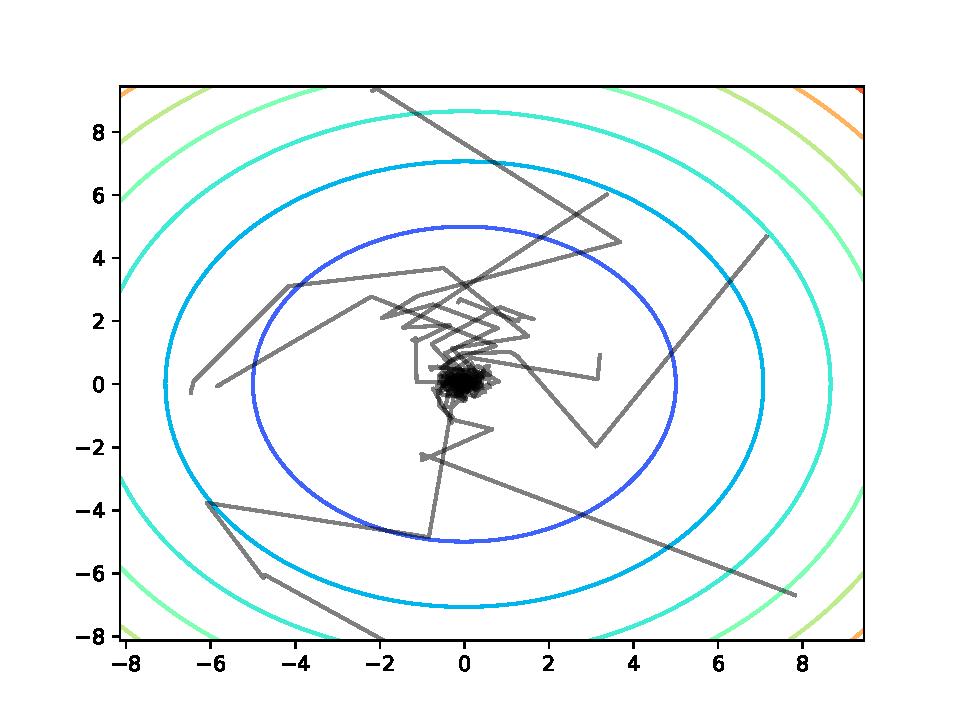
\includegraphics[scale=0.3]{assets/sphere_theta}
    \end{center}
  \column{0.5\textwidth}
    \begin{itemize}
      \item Relatively consistent performance for a convex function.
    \end{itemize}
\end{columns}
\end{frame}

\begin{frame}
\frametitle{Results of Single Bacterium}
\begin{columns}
  \column{0.5\textwidth}
    \begin{center}
      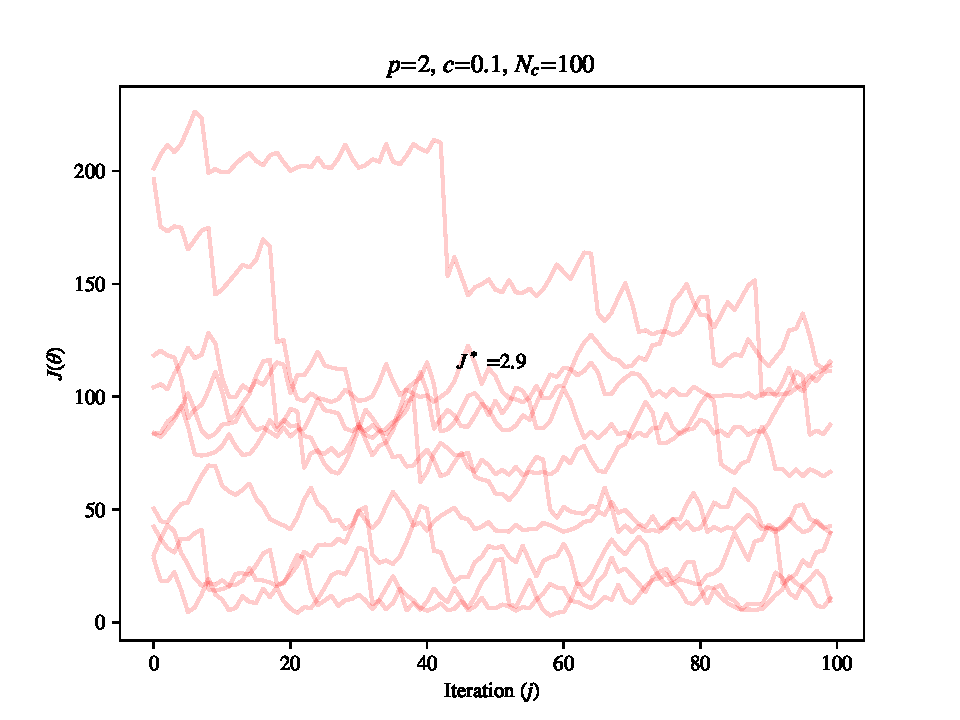
\includegraphics[scale=0.3]{assets/rastrigin_J}
      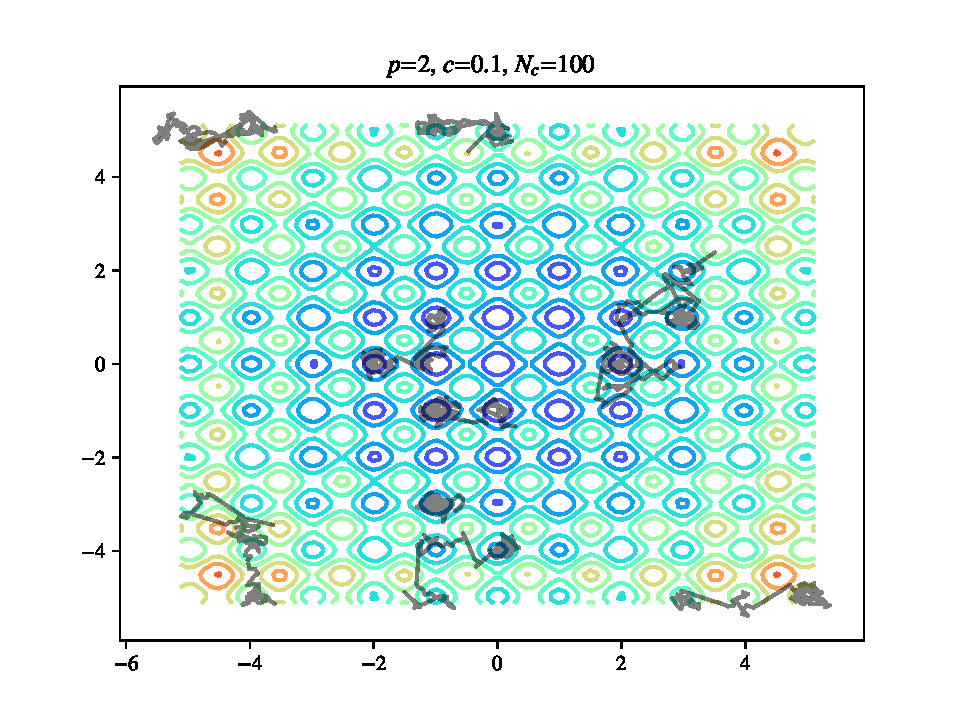
\includegraphics[scale=0.3]{assets/rastrigin_theta}
    \end{center}
  \column{0.5\textwidth}
    \begin{itemize}
      \item Relatively inconsistent performance for a highly nonconvex function.
    \end{itemize}
\end{columns}
\end{frame}

\begin{frame}
\frametitle{Algorithm for a Colony}
\begin{algorithmic}[1]
\For {$j \gets 1 \dots N_c $}:
  \For {$i \gets 1 \dots S$}:
    \State $\phi \sim \mathcal{U}$
    \State $\theta_i \gets \theta_i + c_i \phi$
    \While {$J(\theta_i + c_i \phi) + J_{cc}(\theta_i + c_i \phi) < J(\theta_i) + J_{cc}(\theta_i)$}:
      \State $\theta_i \gets \theta_i + c_i \phi$
    \EndWhile
  \EndFor
\EndFor
\end{algorithmic}
\begin{itemize}
  \item $\theta_i$: $i$th $p$-dimensional vector (randomly initialized)
  \item $S$: number of bacteria in the colony
  \item $c_i$: a step-size for bacterium $i$
\end{itemize}
\end{frame}

\begin{frame}
\frametitle{$J_{cc}$ and swarming behaviour}
\begin{itemize}
  \item \textit{\textit{E. coli}} do social foraging
  \item Secrete a substance to indicate to attract nearby \textit{\textit{E. coli}} and encourage swarming
  \item Strength of signal diffuses over space
  \item Use gaussian distribution to model this
\end{itemize}
\begin{align*}
J_{cc}(\theta) = \sum_{i=1}^S &-d_\text{attract} \exp \left( -w_\text{attract} (\theta - \theta_i)^T (\theta - \theta_i) \right) \\ &+ h_\text{repellant} \exp \left( -w_\text{repellant} (\theta - \theta_i)^T (\theta - \theta_i) \right)
\end{align*}
\end{frame}

\begin{frame}
\frametitle{$J_{cc}$ and swarming behaviour}
\begin{center}
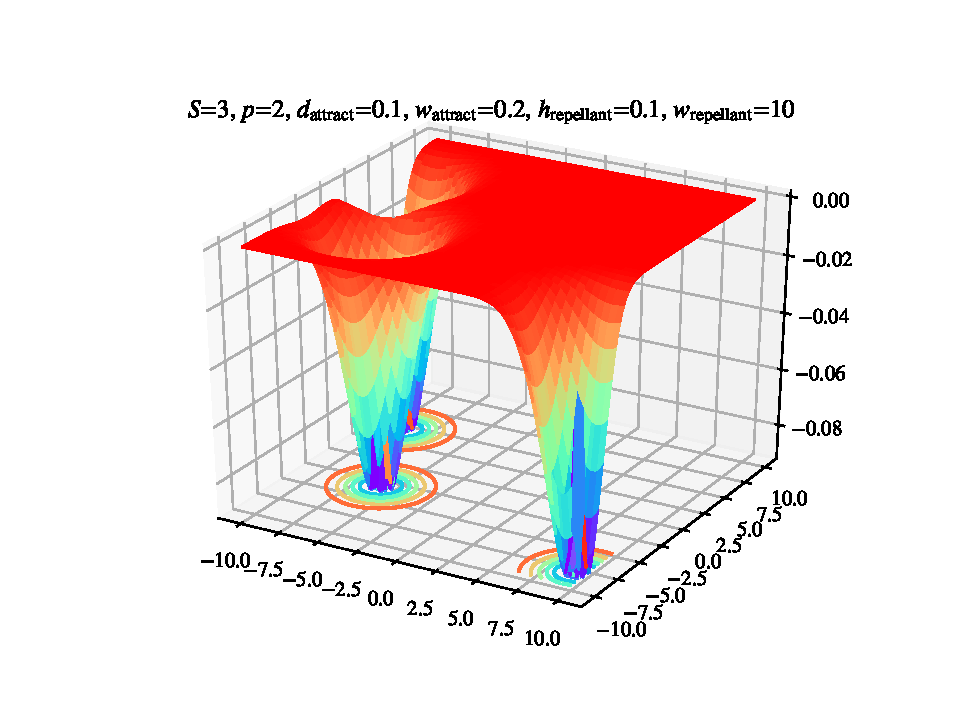
\includegraphics[scale=0.5]{assets/swarming}
\end{center}
\end{frame}

\begin{frame}
\frametitle{Results of Single Bacterium}
\begin{columns}
  \column{0.5\textwidth}
    \begin{center}
      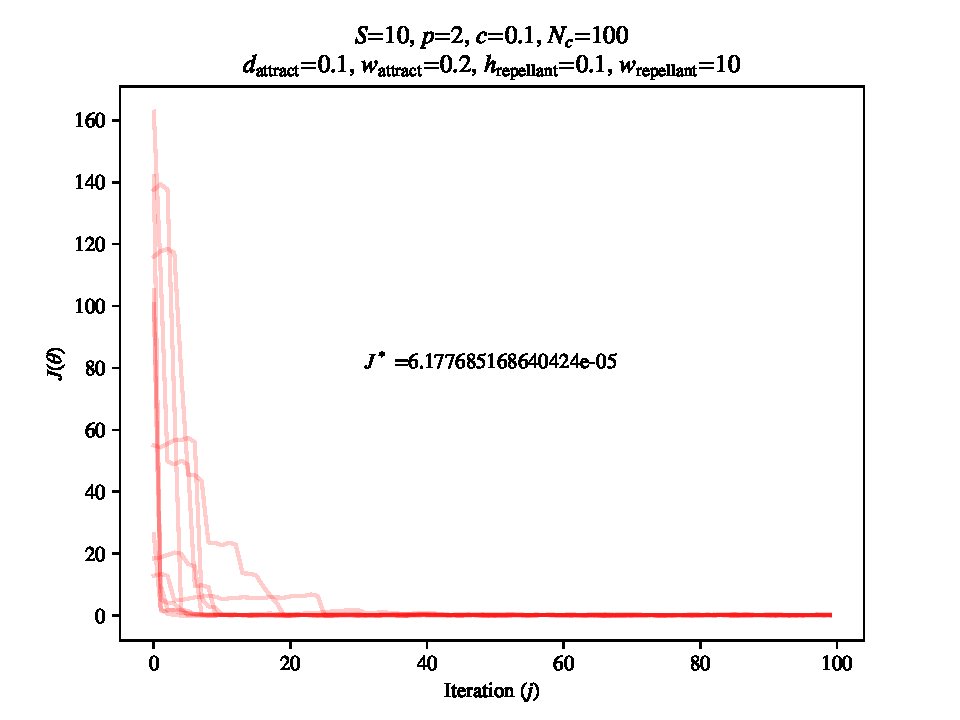
\includegraphics[scale=0.3]{assets/sphere_colony_J}
      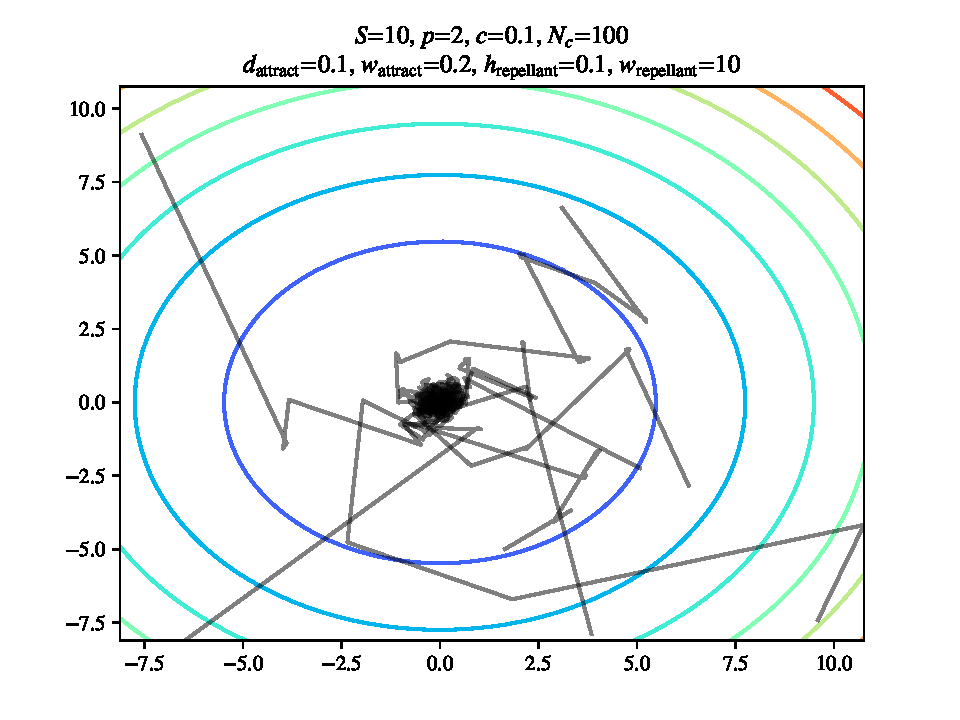
\includegraphics[scale=0.3]{assets/sphere_colony_theta}
    \end{center}
  \column{0.5\textwidth}
    \begin{itemize}
      \item Still relatively consistent performance for a convex function.
      \item Achieves similar performance to single bacterium.
    \end{itemize}
\end{columns}
\end{frame}

\begin{frame}
\frametitle{Results of Single Bacterium}
\begin{columns}
  \column{0.5\textwidth}
    \begin{center}
      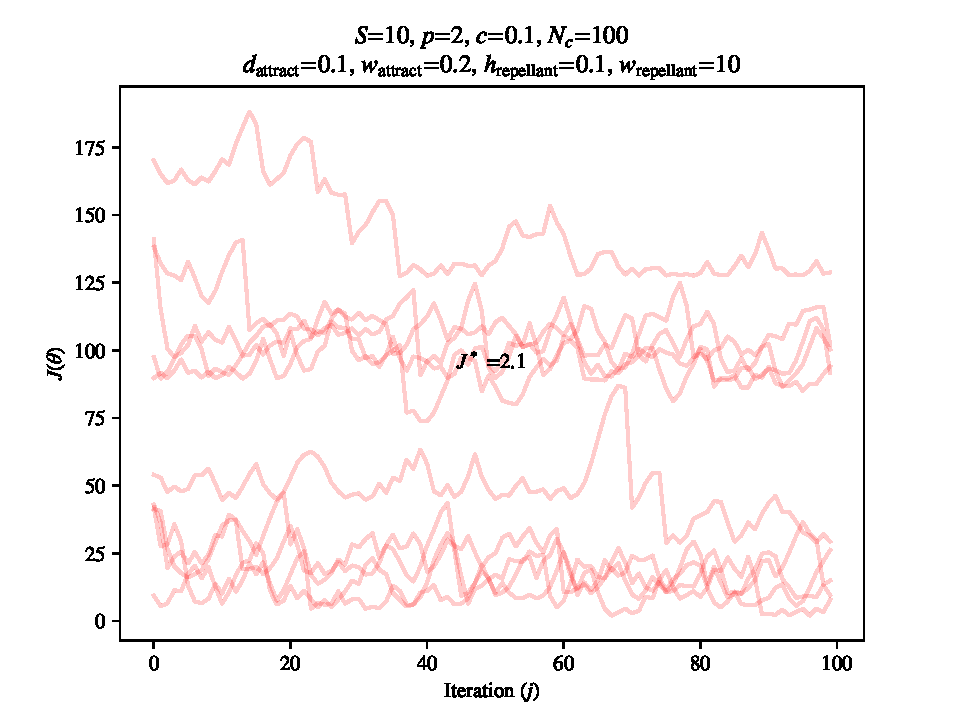
\includegraphics[scale=0.3]{assets/rastrigin_colony_J}
      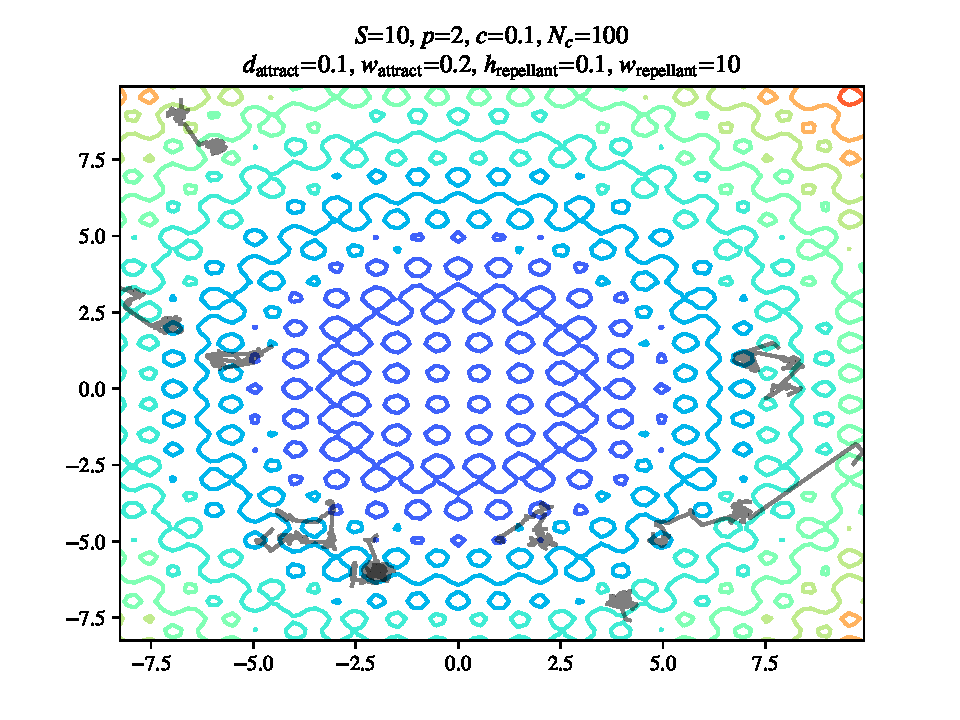
\includegraphics[scale=0.3]{assets/rastrigin_colony_theta}
    \end{center}
  \column{0.5\textwidth}
    \begin{itemize}
      \item Still relatively inconsistent performance for a highly nonconvex function.
      \item But wait... What if the problem is just the hyperparameters?
    \end{itemize}
\end{columns}
\end{frame}

\begin{frame}
\frametitle{Results of Single Bacterium}
\begin{columns}
  \column{0.5\textwidth}
    \begin{center}
      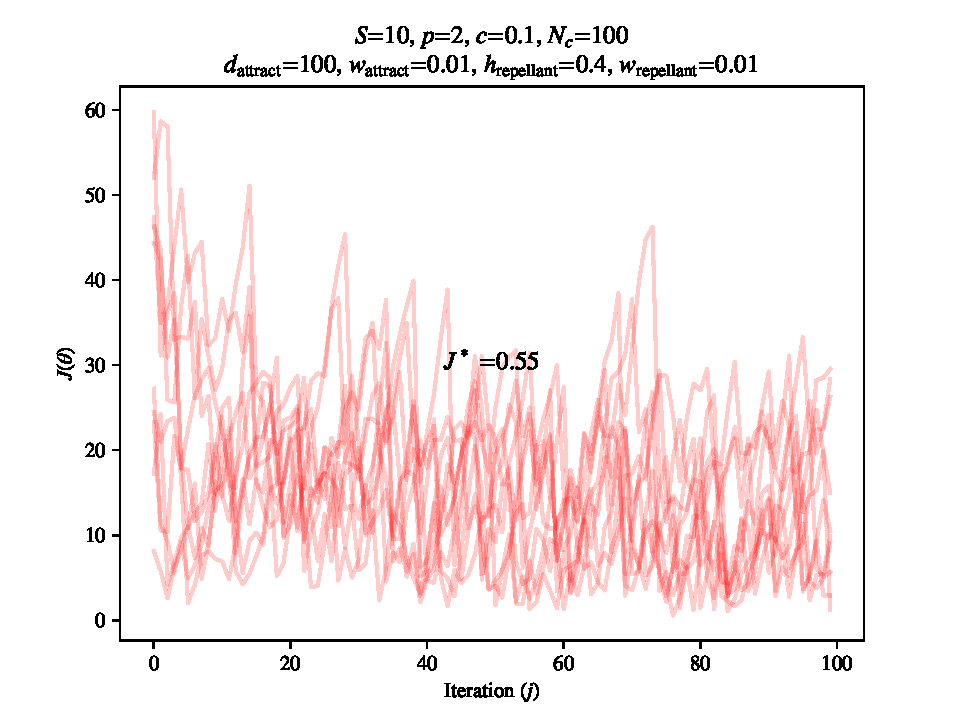
\includegraphics[scale=0.3]{assets/rastrigin_colony_tuned_J}
      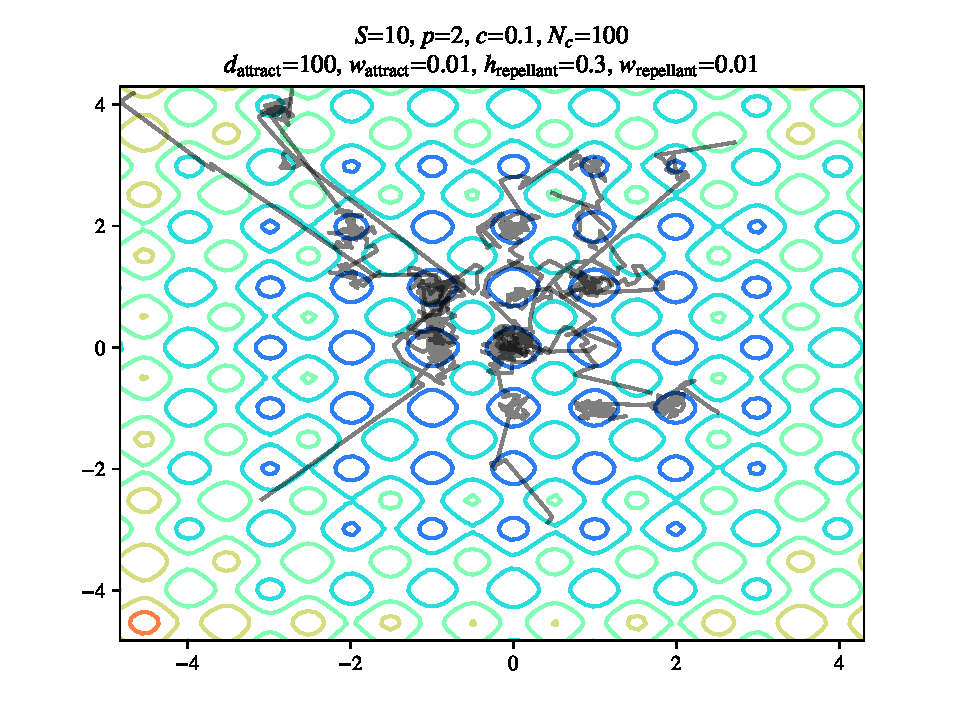
\includegraphics[scale=0.3]{assets/rastrigin_colony_tuned_theta}
    \end{center}
  \column{0.5\textwidth}
    \begin{itemize}
      \item By trying out different combinations of hyperparameters we can improve overall performance.
      \item Here we increased the depth and width of attraction as well as the depth and width of repellance to increase "global" behaviour.
    \end{itemize}
\end{columns}
\end{frame}

\begin{frame}
\frametitle{Algorithm for a Reproducing Colony}
\begin{algorithmic}[1]
\For {$k \gets 1 \dots N_{re}$}:
  \For {$j \gets 1 \dots N_c $}:
    \For {$i \gets 1 \dots S$}:
      \State $\phi \sim \mathcal{U}$
      \State $\theta_i \gets \theta_i + c_i \phi$
      \While {$J(\theta_i + c_i \phi) + J_{cc}(\theta_i + c_i \phi) < J(\theta_i) + J_{cc}(\theta_i)$}:
        \State $\theta_i \gets \theta_i + c_i \phi$
      \EndWhile
    \EndFor
  \EndFor
  \State delete worst $S/2$ and reproduce best $S/2$
\EndFor
\end{algorithmic}
\begin{itemize}
  \item $N_{re}$: number of reproduction steps
\end{itemize}
\end{frame}

\begin{frame}
\frametitle{Algorithm for a Reproducing Colony}

\end{frame}




% cons
% no attempts to compare to actual biological
% does not compare to exissting methods. do you want to be a good optimization algorithm or a good biological model? its neither
% spends long time in introduction describing things like search strategies (cruise, ambush, saltatory), but only ends up using one
% discusses how foraging and looking for nutrients depends on the concentration of nutrients and how the nutrients can be used up, but then ignores this information when desigining the simulation
% do you want a gradient-free hill-climbing algorithm or a simulation of e coli behaviour?
%

\end{document}
